%% Todas as opcoes da classe abnt (AbnTeX) sao validas.
%% Outras opcoes sao: quali e tese (dissertacao e' padrao)
\documentclass[revisao]{ppgccufscar}
%\documentclass[]{abntex2}
% \usepackage{lmodern}			% Usa a fonte Latin Modern	

%% pacotes incompativeis:
%%   qualquer pacote de citacoes, como natbib, apalike, cite, etc.
%% o pacote babel ja vem carregado com ingles e portugues
%\usepackage[brazil]{babel}
%\usepackage[utf8]{inputenc}
\usepackage[latin1]{inputenc}
\usepackage[T1]{fontenc}

\usepackage{upgreek}
\usepackage{mathrsfs}
\usepackage{amsmath}
\usepackage{graphicx}
\usepackage{graphics}

\usepackage{enumerate}
\usepackage{multirow}
\usepackage{verbatim}

\usepackage{indentfirst}% Indenta o primeiro par�grafo de cada se��o.

% Color control.
\usepackage[usenames,dvipsnames]{xcolor}

% Soul package: to use the \hl{} command to highlight text, useful to spot "to-do" items.
% The command \phl is defined so a different highlight color is used by the professor in his/her notes.
\usepackage{soul}
%\usepackage{soulutf8}
\newcommand{\phl}[2][Peach]{{\sethlcolor{#1} \hl{#2}}}

%%%%%%%%%%%%%%%%%%%%%%%%%%%%%%%%%%%%%%%%%%%%%%%%%%%%%%%%%%%%%%%%%%%%%%%% 
% Definitions

\graphicspath{{../../images/}}

%\bibliographypath{{../../references/}}

\newtheorem{mydef}{Defini\c{c}\~ao}

\newenvironment{bigequation}{\begin{equation} \fontsize{16pt}{20pt}}{\end{equation}}

\newcommand{\cc}[2][c]{%
	\begin{tabular}[#1]{@{}c@{}}#2\end{tabular}}


%%%%%% Titulo PDF
\title{Revisao leo}

%%%%%%%%%%%%%%%%%%%%%%%%%%%%%%%%%%%%%%%%%%%%%%%%%%%%%%%%%%%%%%%%%%%%%%%%
% Altere os campos abaixo para alterar o documento final
%%%%
\titulo { Trabalho de conclus�o da mat�ria de revis�o sistem�tica }
%%%%
\autor{Leonardo Almeida Silva Ferreira}
%%%%
\orientador[Orientadora]{Profa. Dra. Eloize Rossi Marques Seno}
%%%%
%\coorientador{Prof. Dr. XXXX}
%%%%
\areaconcentracao{Revis�o Sistem�tica}
%%%%
\data{Abril/2017}
%%%%
\instituicao{Instituto Federal de Educa\c{c}\~ao Ci\^encia e Tecnologia de S\~ao Paulo -- Campus S\~ao Carlos}
%%%%
\local{S\~ao Carlos -- SP}
%%%%
\comentario{\PPGtipodoc\ apresentada no Curso de Especializa\c{c}\~ao Lato Sensu em Desenvolvimento de Sistemas para Dispositivos M\'oveis do Instituto Federal de Ci\^encia e Tecnologia de S\~ao Paulo - Campus de S\~ao Carlos, como parte dos requisitos para a obten\c{c}\~ao do t\'{\i}tulo de \PPGtipotitulo\ em desenvolvimento de sistemas para dispositivos m\'oveis.}
%%%%
\instituicaodetails{}
%%%%%%%%%%%%%%%%%%%%%%%%%%%%%%%%%%%%%%%%%%%%%%%%%%%%%%%%%%%%%%%%%%%%%%%%

% epigrafre, agradecimentos sao feitos 'na mao'.
% um dia eu faco alguns comandos para eles ;)

\begin{document} 
	
\capa
\folhaderosto
%\folhadeaprovacao
%\endfolhadeaprovacao

%\dedicatoria{A meus pais.}
%\begin{agradecimentos}
Agradeço ao \LaTeX por não ter vírus de macro.
Agradeço ao Linus Torvalds por ter feito o Linux.
Agradeço ao Bill Gates por deixar-nos piratear seus softwares.
\end{agradecimentos}

%\epigrafe{Um dia.}{Dadavski Shoffstall}

\begin{resumo}
	Nonono nonono nonono, nonono, nonono nonono nonono nononono nonno.
	Nonono nonono nonono, nonono, nonono nonono nonono nononono nonno.
	Nonono nonono nonono, nonono, nonono nonono nonono nononono nonno.
	Nonono nonono nonono, nonono, nonono nonono nonono nononono nonno.
	Nonono nonono nonono, nonono, nonono nonono nonono nononono nonno.
	Nonono nonono nonono, nonono, nonono nonono nonono nononono nonno.
	Nonono nonono nonono, nonono, nonono nonono nonono nononono nonno.


\palavraschave{
	Computa\c{c}\~{a}o M\'{o}vel,  
	Comunica\c{c}\~{a}o sem Fio, 
	Comunica\c{c}\~{a}o Oportun\'{i} stica }
\end{resumo}

\begin{abstract}
Nonono nonono nonono, nonono, nonono nonono nonono nononono nonno.
Nonono nonono nonono, nonono, nonono nonono nonono nononono nonno.
Nonono nonono nonono, nonono, nonono nonono nonono nononono nonno.
Nonono nonono nonono, nonono, nonono nonono nonono nononono nonno.
Nonono nonono nonono, nonono, nonono nonono nonono nononono nonno.
Nonono nonono nonono, nonono, nonono nonono nonono nononono nonno.
Nonono nonono nonono, nonono, nonono nonono nonono nononono nonno.

\keywords{
	Computa\c{c}\~{a}o M\'{o}vel,  
	Comunica\c{c}\~{a}o sem Fio, 
	Comunica\c{c}\~{a}o Oportun\'{i} stica }
\end{abstract}


\listoffigures
\listoftables

%% sumario
\tableofcontents

%% aqui comeca o texto da disserta��o


\chapter{Introdu\c{c}\~{a}o/motiva\c{c}\~{a}o}
Muitas vezes ao pensar em internet das coisas (IoT), contextualizando seu impacto na intera\c{c}\~{a}o entre pessoas e o ambiente ao seu redor, \'{e} enfatizado o uso de informa\c{c}\~{o}es traduzidas do ambiente (temperatura, humidade e etc.) para automatiza\c{c}\~{a}o, controle ou qualquer tomada de decis\~{a}o. Contudo, a inclus\~{a}o de informa\c{c}\~{o}es proveniente das redes sociais, estruturando um senso comum, se torna um fator de grande impot�ncia na forma\c{c}\~{a}o de uma opini\~{a}o acertiva em rela\c{c}\~{a}o aos acontecimentos perif\'{e}ricos ao nosso foco principal.

O objetivo principal desse estudo \'{e} estruturar o conceito de Internet das Coisas e suas deriva\c{c}\~{o}es, cujo primeiro passo para uma efetiva implanta\c{c}\~{a}o \'{e} criar nas pessoas envolvidas um bom entedimento sobre seus conceitos. Contudo, em uma breve revis\~{a}o da literatura existente no mundo podemos verificar o qu\~{a}o controverso s\~{a}o esses conceitos. A proposta desse documento \'{e} apresentar alguns fatos desde a origem do conceito at\'{e} os dias atuais de forma a facilitar o entendimento do assunto. Sob um diferente ponto de vista, pretendo demonstrar a cont\'{i}gua rela\c{c}\~{a}o de conceitos da Internet das Coisas com outros termos como Computa\c{c}\~{a}o Ub\'{i}qua, Disappearing Computer e Web das Coisas e Web Social das Coisas.

A segunda parte, busca apresentar brevemente algumas das tecnologias que est\~{a}o fortalecendo o conceito de Internet das Coisas e devem conduzir seu futuro.

Esse artigo busca ajudar no entedimento sobre alguns conceitos b\'{a}sicos sobre Internet das Coisas, a origem desse paradigma, pontuando semelhan\c{c}a com outros conceitos e por fim apresentando algumas das tecnologias que est\~{a}o aparecendo para definir a base do ecossistema da Internet das Coisas e ferramentas importantes no processo de minera\c{c}\~{a}o dos dados provenientes de dispositivos conectados.

	\section{Das origens � Web Social das Coisas}
	Considerando o quanto o termo Internet das Coisas \'{e} utilizado em nosso dia-a-dia de trabalho e pesquisa, juntando ao fato de que esse termo \'{e} bastante controverso na literatura de computa\c{c}\~{a}o, sendo at\'{e} mesmo confundido com outros termos, penso que a melhor forma de iniciarmos a sua compreens\~{a}o seria entendendo seu atual momento e identificando fatos do passado que a levaram aos seus padr\~{o}es atuais de funcionamento. 
	
	Como fatos relevantes, entendo que eventos motivadores de sua cria\c{c}\~{a}o, de seus termos e objetivos s\~{a}o de grande importancia, assim como o fato que conduziu seus idealizadores a escolha dos padr\~{o}es atuais em detrimento de outros existentes e desafios ou necessidades do passado que motivaram mudan\c{c}as nos seus objetivos.
	
	At\'{e} a d\'{e}cada de 60, ocorreram diversos fatos relacionados � cria\c{c}\~{a}o e expan\c{c}\~{a}o das telecomunica\c{c}\~{o}es no mundo, fatos que n\~{a}o s\~{a}o o foco desse artigo. Ap\'{o}s esse per\'{i}odo de evolu\c{c}\~{a}o das comunica\c{c}\~{o}es, que os cientistas come\c{c}aram os debates sobre como seria se grande parte do mundo que vivemos pudesse ser virtualizado, sendo esses debates um press\'{a}gio para a Internet das coisas.
	
		\paragraph{Anos 60}
		Em seu livro "Understanding Media" McLuhan~\cite{McLuhan1964} descrevia que por meio de m\'{i}dias eletr\^{o}nicas, eles haviam configurado uma din�mica onde todas as tecnologias anteriores (incluindo as cidades como conheciam) seriam traduzidas em sistemas de informa\c{c}\~{a}o. Nos anos seguintes Karl Steinbuch~\cite{KlausBiener1997}. No fim da d\'{e}cada foi criada a Arpanet, primeira rede computadores, iniciando o ciclo de desenvolvimento da internet ~\cite{MichaelHAUBEN1995}. 
		
		\paragraph{Anos 80}
		O DNS(Domain Name System) foi criado para facilitar o acesso � internet atrav\'{e}s de dom\'{i}nios no lugar dos n\'{u}meros IP ~\cite{Mockapetris1983}, enquanto que Tim Berners-Lee fez a proposta de cria\c{c}\~{a}o da rede mundial de computadores~\cite{Berners-Lee1989}.
		
		No final desse per\'{i}odo, Mark Weiser(CTO da Xerox PARC) criou o projeto Computa\c{c}\~{a}o Ub\'{i}qua visando responder rapidamente erros do conceito de computador pessoal: alta complexidade; dif\'{i}cil de utilizar; exige demais a aten\c{c}\~{a}o dos usu\'{a}rios; isola muito as pessoas do mundo; e excessivamente dominante, por ocupar muito a vida e mesa de trabalho das pessoas~\cite{Weiser1999}.
		
		\paragraph{Anos 90}
		Com a rede mundial de computadores ainda embrion\'{a}ria, o conceito de Internet das Coisas come\c{c}ou a se formar partindo da torradeira criada por John Romkey, tendo em vista a demonstra\c{c}\~{a}o que ele e seus colegas fariam na confer\^{e}ncia INTEROP para apresentar o protocolo de rede SNMP que estavam criando naquele momento ~\cite{Romkey2017}. Esse se tornou o primeiro dispositivo IoT, que conectada a um computador em rede e usando uma base de informa\c{c}\~{a}o (SNMP MIB), pode ligada e desligada remotamente.
		
		Nesse per\'{i}odo, Mark Weiser com suas publica\c{c}\~{o}es, definiu alguns dos principais conceitos da Internet das Coisas. Inicialmente em seu primeiro artigo sobre o assunto ele define a Computa\c{c}\~{a}o Ub\'{i}qua como tecnologias que desaparecerem, compostas por elementos delas mesmas na ess\^{e}ncia da vida cotidiana at\'{e} se tornarem igualmente impercept\'{i}veis a si pr\'{o}prias~\cite{Weiser1991}, alguns anos depois em outro artigo ele define a computa\c{c}\~{a}o Ub\'{i}qua como o oposto da realidade virtual, onde de um lado as pessoas s\~{a}o conduzidas a um mundo criado por computadores, do outro \'{e} institu\'{i}do �s m\'{a}quinas que coabitem com as pessoas no mundo real ~\cite{Weiser1993}. Em um terceiro artigo, ao descrever um projeto de circuito el\'{e}trico criado por sua colega de empresa, Weiser cunhou "Tecnologias Calmas" ou "Intelig\^{e}ncia ambiental" com a seguinte frase: "N\~{a}o requer nenhum espa\c{c}o na tela do seu computador e de fato n\~{a}o usa ou comp\~{o}es computadores. N\~{a}o utiliza softwares, somente alguns d\'{o}lares em hardware e pode ser compartilhado por v\'{a}rias pessoas ao mesmo tempo." ~\cite{Weiser:1997:CAC:504928.504934}.
		
		Ao criar o 'Trojan Room Coffee Pot' para monitorar a quantidade de caf\'{e} da m\'{a}quina do laborat\'{o}rio de computa\c{c}\~{a}o da Universidade de Cambridge, Quentin Stafford-Fraser e Paul Jardetzky acabaram por criar o que podemos considerar como um dos prim\'{o}rdios do IoT. Se tratava de uma camera que mantinha atualizado nos servidores do pr\'{e}dio, imagens (3 por minuto) da m\'{a}quina de caf\'{e} para que as pessoas pudessem consultar se tinha caf\'{e}, evitando uma viagem perdida ~\cite{Stafford-Fraser1995}. Na mesma \'{e}poca foi criada a WearCam por Steve Mann, considerada o primeiro "Wearable" ~\cite{SteveMann1995}.
		
		Quando Paul Saffo publicou o artigo "Sensors: The Next Wave of Infotech Innovation"~\cite{Saffo:1997:SNW:253671.253734}, ele descreveu os motivos que fariam dos sensores ubiquos a pr\'{o}xima onda de inova\c{c}\~{a}o concluindo que num futuro pr\'{o}ximo, sensores anal\'{o}gicos seriam facilmente interligados � computadores digitais e � redes de computadores criando uma rede de sensores. Comprovando essa tese, o projeto inTouch ~\cite{Brave:1997:IMH:1120212.1120435} criou uma tecnologia chamada de "telefone tang\'{i}vel", que sincroniza objetos f\'{i}sicos de forma distribu\'{i}da utilizando sensores para comunica\c{c}\~{a}o t\'{a}til � longa dist�ncia.
		
		Em 1999, Kevin Ashton criou o termo Internet das Coisas ao descrever um sistema onde a internet \'{e} conectada ao mundo real utilizando diversos sensores ubiquos. Ashton~\cite{Ashton2009} cita como acontenceu, em seu artigo: "Poderia estar errado, mas eu estou certo que o termo Internet das Coisas teve inicio como t\'{i}tulo de uma apresenta\c{c}\~{a}o feita por mim na Procter \& Gamble em 1999. Ao unir a nova ideia de utiliza\c{c}\~{a}o do RFID na cadeia de suprimentos da P\&G aos t\'{o}picos acalorados at\'{e} ent\~{a}o sobre Internet foi uma forma encontrada de chamar a aten\c{c}\~{a}o dos executivos. Isso elucida algo que habitualmente cria um mal entendido."
		
		\paragraph{Anos 2000}
		
		Com a dissemina\c{c}\~{a}o do termo Internet das Coisas, ele passa a ser mencionado inumeras vezes em publica\c{c}\~{o}es convencionais, como The Guardian, Scientific American e The Boston Globe e pela primeira vez come\c{c}a a aparecer nos t\'{i}tulos de livros. Come\c{c}am a aparecer projetos visando a implementa\c{c}\~{a}o de algumas das ideias propostas, como o Cooltown, o Internet0 e a iniciativa "Disappearing Computer".
		
		A tecnologia RFID come\c{c}a a ser implementada em larga escala pelo departamento de defesa americano nos programas de combate � viol\^{e}ncia sexual (Savi Program) e comercialmente pelo Walmart em suas pr\'{o}prias lojas. 
		
		A Internet das Coisas come\c{c}a a se consolidar quando a Uni\~{a}o Europ\'{e}ia, reconhece a import�ncia acad\^{e}mica do assunto sediando sua primeira confer\^{e}ncia internacional e a Uni\~{a}o Internacional de Telecomunica\c{c}\~{o}es (ITU) publica seu primeiro relat\'{o}rio com a seguinte afirma\c{c}\~{a}o: "Uma nova dimens\~{a}o tem sido inclu\'{i}da no mundo das tecnologias da informa\c{c}\~{a}o e comunica\c{c}\~{a}o (ICTs): A qualquer hora, as pessoas podem se conectar em qualquer lugar, agora teremos conectividade em tudo. As conex\~{o}es ir\~{a}o se multiplicar e criar uma din�mica inteiramente nova de rede de redes - uma Internet das Coisas" ~\cite{ITU2005}.
		
		Seu reconhecimento internacional incentivou um grupo de empresas da \'{a}rea de tecnologia, comunica\c{c}\~{o}es e energia fundar a IPSO Alliance para promo\c{c}\~{a}o da utiliza\c{c}\~{a}o do protocolo IP em redes de objetos inteligentes. Al\'{e}m das empresas, muitos governos tamb\'{e}m mostraram grande interesse na nova ind\'{u}stria, principalmente a china ao injetar grande quantidade de recursos nos fundos de pesquisas de suas principais instituti\c{c}\~{o}es ~\cite{Zhengyan2009}. De forma a viabilizar o avan\c{c}o de pesquisas em novas tecnologias, o FCC liberou a utiliza\c{c}\~{a}o dos espa\c{c}os sem uso entre as frequ\^{e}ncias 470 MHz e 698 MHz. 
		
		Com pesquisas sendo realizadas nos 4 cantos do mundo, o Conselho Nacional de intelig\^{e}ncia Americano lista a Internet das Coisas como uma das 6 Tecnologias civ\'{i}s disruptivas com potencial impacto nos interesses Americanos at\'{e} o ano de 2025 e pesquisa citada em ~\cite{Evans2011} mostra que a quantidade de "objetos ou coisas" (em referencia aos dispositivos m\'{o}veis) conectados � internet j\'{a} atingiam 12.5 bilh\~{o}es em 2010, enquanto que a popula\c{c}\~{a}o chegava a 6.8 bilh\~{o}es de pessoas no mundo, al\c{c}ando o patamar de 1,84 dispositivos conectados por pessoa. 
		
		Prevendo a incapacidade do IPv4 em atender a acentuada expans\~{a}o na conex\~{a}o de equipamentos � internet a IETF (Internet Engineering Task Force) lan\c{c}ou ao p\'{u}blico o padr\~{a}o IPV6 ~\cite{WORLDIPV62012} permitindo a conex\~{a}o de aproximadamente 340 undecilh\~{o}es de endere\c{c}os ou como apontado por Steven Leibson, "Podemos assinalar um endere\c{c}o IPV6 para cada \'{a}tomo na superf\'{i}cie da terra e ainda assim teremos endere\c{c}os suficientes para endere\c{c}amento de outros 100 ou mais planetas terra.".
		
		De forma a promover uma abordagem universal no desenvolvimento de padr\~{o}es t\'{e}cnicos, a Uni\~{a}o Internacional de Telecomunica\c{c}\~{o}es cria o grupo de estudos IoT-GSI(depois transformado em SG20), pemitindo um alcance global � Internet das Coisas. No ramo dos neg\'{o}cios, o instituto de pesquisa gartner inclui o termo Internet das Coisas em seu Hype Cycle anual, respons\'{a}vel pelo rastreamento do ciclo de vida das tecnologias da sua apari\c{c}\~{a}o ao seu plat\^{o} de produtividade. A Internet das Coisas atinge seu pico de expectativa em 2014 segundo o instituto.
		
		Iniciativas educacionais e de marketing sobre o t\'{o}pico come\c{c}am a ser produzidos em larga escala por grandes empresas e comunidades nas redes sociais relacionada �s Internet das Coisas como Linkedin e a plataforma de "networking" \_connect do Conselho de Estrat\'{e}gia Tecnol\'{o}gica do Reino Unido.
		
		O amadurecimento das plataformas de prototipa\c{c}\~{a}o (Arduino) e dos computadores baseados em SoC (Raspberry Pi, Intel Edison) permitiu aos entusiastas investir na cria\c{c}\~{a}o de pequenos projetos de forma acess\'{i}vel e com isso verificamos uma expans\~{a}o na quantidade de plataformas (Pachube e Thingspeak), padr\~{o}es de protocolos (6LoWPAN, Dash7, etc), Sistemas Operacionais (Contiki, TinyOS, etc) que est\~{a}o sendo desenvolvidas espec\'{i}ficamente para dar forma ao ecossistema da Internet das Coisas. � com foco nesse ecossistema que empresas especializadas em suas sub-\'{a}reas j\'{a} est\~{a}o se formando como a Mocano, especializada em seguran\c{c}a para IoT.
		
		\paragraph{A partir de 2015}
		Com a socializa\c{c}\~{a}o da internet, o aumento de dispositivos inteligentes conectados e a experi\^{e}ncia dos usu\'{a}rios com os impactos das novas tecnologias na vida das pessoas, era de se esperar que disrupturas ao redor da "Intenet das Coisas" acontecessem. De acordo com ~\cite{Mashal2015} atuamente est\~{a}o alta pesquisas relacionadas aos conceitos da Web das Coisas (WoT) focando na reutiliza\c{c}\~{a}o de padr\~{o}es abertos da internet atual na interoperabilidade entre dispositivos inteligentes ao compartilhar as informa\c{c}\~{o}es coletadas por sensores ub\'{i}quos e da Web Social das Coisas (SWoT) ressaltando o estudo de novas formas para integrar dispositivos inteligentes ("smart things") entre eles e com os humanos, mas n\~{a}o apenas como ponte entre a realidade e o virtual, mas fazendo parte do mundo real, pondendo atuar como tomador de decis\~{o}es em favor das pessoas se necess\'{a}rio. Essa abordagem futur\'{i}stica da SWoT, baseada em conceitos de tecnologias calmas e redes sociais, faz dela a mais promissora atualmente com a consolida\c{c}\~{a}o da Internet das Coisas, se tornando uma \'{a}rea de pesquisas atualmente ativa.
		
		
		%% Incluir parte sobre WIoT, Edge Computing, CoT, Objetos Virtuais


\chapter{Contextos envolvidos}

\section{Computa\c{c}\~{a}o ub\'{i}qua �  SIoT}
	\subsection{Computa\c{c}\~{a}o Ub\'{i}qua}
	A computa\c{c}\~{a}o ubiqua deu nome � terceira onda da computa\c{c}\~{a}o, iniciada por Mark Weiser em seu artigo ~\cite{Weiser1991}. Segundo outro artigo de sua autoria, ele~\cite{Weiser:1997:CAC:504928.504934} define a terceira onda da computa\c{c}\~{a}o assim; 
	"...Esse terceiro momento ocorre quando as tecnologias recuam para o segundo plano de nossas vidas e muitos computadores (n\~{a}o apenas um) de forma conjunta passam a exercer um papel auxiliar para as pessoas sem tomar tempo do foco principal de sua aten\c{c}\~{a}o.
	
	O principal objetivo das pesquisas na \'{a}rea da computa\c{c}\~{a}o ub\'{i}qua s\~{a}o relacionadas ao refinamento dos dispositivos eletr�nicos de forma que sua utiliza\c{c}\~{a}o seja efetiva e eficiente na cria\c{c}\~{a}o de um contexto computacional~\cite{VanSyckel:2014:SPP:2638728.2641672}, seria como criar uma "conci�ncia virtual" para esse dispositivos de forma que sua utiliza\c{c}\~{a}o possa se tornar transparente para as pessoais. 
	
	Infelizmente, para grande parte das aplica\c{c}\~{o}es nesse paradigma, operar seus dispositivos inteligentes de forma transparente �s pessoas significa ter acesso a informa\c{c}\~{o}es altamente sens\'{i}veis de individuos, exigindo que esses dispositivos sejam projetados cuidadosamente de forma a n\~{a}o se tornar um sistema de fiscaliza\c{c}\~{a}o. Por outro lado, sistemas ub\'{i}quos precisam ser fortemente examinados sobre uma perspectiva de ataques cibern\'{e}ticos, pois j\'{a} se sabe de antem\~{a}o o qu\~{a}o valiosa s\~{a}o suas infoma\c{c}\~{o}es, suscitando grande interesse \'{a} pessoas mal-intencionadas.
	
	\subsection{Disappearing Computer}
	Baseado nas defini\c{c}\~{o}es de Weiser sobre Computa\c{c}\~{a}o Ub\'{i}qua ~\cite{Weiser1991}, surgiu a necessidade de ampliar as pesquisas em tecnologias que fazem dos computadores objetos impercept\'{i}veis, ficando apenas em segundo plano sem tirar o foco das pessoas. A partir dessa disruptura nasceu o termo "Disappearing Computer" com a distin\c{c}\~{a}o dos dispositivos invis\'{i}veis em 2 tipos Desaparecimento F\'{i}sico e Desaparecimento Mental como descrito por Streitz em ~\cite{streitz2001augmented}. 
	
	\paragraph{Desaparecimento F\'{i}sico}
	Como o nome j\'{a} diz, um dispositivo computacional desaparece f\'{i}sicamente, quando ele \'{e} t\~{a}o pequeno que cabe na palma da m\~{a}o, podendo ser costurado em tecidos, colocado junto ao corpo das pessoas ou mesmo implantado no corpo. Na maior parte dos casos, o dispositivo \'{e} integrado � um produto de pequena dimens\~{a}o onde seus recursos computacionais se tornam invis\'{i}veis.
	
	\paragraph{Desaparecimento Mental}
	O aspecto essencial desses cen\'{a}rios \'{e} projetar os dispositivos de forma a n\~{a}o serem mais percebidos como computadores e sim como mais um dos elementos que comp\~{o}e aquele ambiente. Aqui o desaparecimento se limita aos olhos de seus usu\'{a}rios. O dispositivo n\~{a}o precisa ser invis\'{i}vel fisicamente, ele pode estar embutido em portas, janelas e mobili\'{a}rios ou ter apenas sua apar�ncia modificada, dando naturalidade ao inclu\'{i}-lo no ambiente com sua nova roupagem e ficando oculto ao olhar humano.
	
	\subsection{Internet das Coisas - IoT}
	Prop\~{o}e um ecossistema de "coisas" interconectadas. Se entende por "coisa", objetos geralmente compostos por pequenos sistemas computacionais embarcados que contam com a habilidade de captar dados do ambiente em an\'{a}lise trocando informa\c{c}\~{a}o com outras "coisas" diretamente ou atrav\'{e}s de uma rede.
	
	Sua principal caracter\'{i}stica que acaba inviabilizando uma implanta\c{c}\~{a}o universal da Internet das Coisas nos dias atuais \'{e} quanto a forma de busca e comunica\c{c}\~{a}o entre os diversos dispositivos ub\'{i}quos dispon\'{i}veis na rede, que deve ser baseado em um identificador \'{u}nico dentro na rede (ex: Seu IP) ou seja, cada "coisa" conectada � rede ter\'{a} que possuir seu identificador pr\'{o}prio. Por\'{e}m, enquanto a migra\c{c}\~{a}o do protocolo IPv4 para o IPv6 n\~{a}o se concretizar, ser\'{a} econ�micamente invi\'{a}vel implementar um ecossistema novo para a Internet das Coisas que seja amplamente universal. Fora isso, como essa caracter\'{i}stica n\~{a}o \'{e} a \'{u}nica, e novas tecnologias continuam sendo pesquisadas e lan\c{c}adas no mercado, nada impede que sejam feitas adapta\c{c}\~{o}es nas redes existentes para alcan\c{c}ar implementa\c{c}\~{o}es baseadas na Internet das Coisas. A mais promissora delas \'{e} a "Web das Coisas" cujo ecossistema \'{e} baseado em protocolos da Web existentes e que j\'{a} est\~{a}o consolidados, como detalhado no pr\'{o}ximo item.
	
	\subsection{Web das Coisas - WoT}
	A partir de um consenso onde a rede mundial de computadores seria a mais vi\'{a}vel para criar uma Internet das Coisas universalizada, apareceram diversas pesquisas com esse objetivo e continuam aparecendo. Por\'{e}m, a ades\~{a}o ao novo protocolo de roteamento (IPv6) com identificadores \'{u}nicos para todos os dispositivo, primordial para sua consolida\c{c}\~{a}o, n\~{a}o est\'{a} ocorrendo com a velocidado prevista criando um hiato na universaliza\c{c}\~{a}o da internet das coisas, j\'{a} que o protocolo atual (IPv4) n\~{a}o \'{e} adequado a essa nova realidade por sua escassez de identificadores.
	
	Como esse processo de migra\c{c}\~{a}o ser\'{a} lento, pesquisadores e empresas iniciaram suas pesquisas utilizando as estruturas da Web atual, adaptando formas de identificar os elementos dentro da rede. O maior avan\c{c}o na dire\c{c}\~{a}o de criar um elo entre os mundos f\'{i}sicos e virtuais veio da ramifica\c{c}\~{a}o de IoT chamada de "Web das Coisas", que utiliza tecnologias da Web (web services, web sockets e etc.) na identifica\c{c}\~{a}o e comunica\c{c}\~{a}o entre os elementos de uma mesma rede de sensores ub\'{i}quos. Dessa forma, a proposta seria que a manuten\c{c}\~{a}o das redes baseadas na "Web das Coisas" n\~{a}o seja afetada com o fim da migra\c{c}\~{a}o para o protocolo IPv6, havendo uma conviv�ncia harm�nica entre as novas redes de dispositivos e que as novas tecnologias criadas para a Web das Coisas possam ser migradas sem traumas para a Internet das Coisas.
	
	Ainda que a causa principal dessa ramifica\c{c}\~{a}o seja o avan\c{c}o na aplica\c{c}\~{a}o das novas tecnologias, ao avaliar t\'{e}cnicamente a comunica\c{c}\~{a}o entre os diversos dispositivos inteligentes existentes atualmente, vemos que h\'{a} uma grande heterog�neidade de implementa\c{c}\~{o}es, resultando em uma complexidade excessiva para firmar essa comunica\c{c}\~{a}o. Em um futuro pr\'{o}ximo, a falta de um protocolo unificado para troca de mensagens inviabilizaria uma intera\c{c}\~{a}o transparente entre esses dispositivos inteligentes. Na solu\c{c}\~{a}o desse problema, a incorpora\c{c}\~{a}o de mecanismos utilizados na cria\c{c}\~{a}o dos Web Services pela internet tem sido estudada para viabilizar a cria\c{c}\~{a}o de uma conex\~{a}o espont�nea entre os dispositivos inteligentes, apenas fazendo adequa\c{c}\~{o}es necess\'{a}rias � nova realidade da Web das Coisas.
	
	%Inclus\~{a}o de Web Sockets e outras tecnologias web
	
	\subsection{Web Social das Coisas - SWoT}
	Esse paradigma, o mais embrion\'{a}rio dentre os que possuem como origem a Computa\c{c}\~{a}o Ub\'{i}qua, real\c{c}a as pesquisas no campo da intelig�ncia computacional e o aspecto social na comunica\c{c}\~{a}o entre usu\'{a}rios, incluindo dispositivos ub\'{i}quos no relacionamento. Sugundo ~\cite{Mashal2015}, esse relacionamento pode ser atingido com a utiliza\c{c}\~{a}o da Web Sem�ntica e tradu\c{c}\~{a}o de dados estruturados em linguagem natural. Por\'{e}m, precisam ser prospostas novas formas dos dispositivos ub\'{i}quos interpretarem as redes de relacionamento existentes criando uma comunica\c{c}\~{a}o transparente entre dispositivos e se comunicando de forma natural e n\~{a}o intrusiva de forma que eles sejam devidamente compreendidos pelas pessoas.
	

\section{Edge computing e o surgimento da Fog computing}
\subsection{sub-item x}

\section{Cloud of Things and Social Cloud}
\subsection{sub-item x}

\section{Social Virtual Objects}
\subsection{sub-item x}

\section{Web Sem�ntica e Ontologias de IoT}
\subsection{sub-item x}

\section{Mundo de IoT e Minera\c{c}\~{a}o de dados}
Mesmo que pesquisas nesse assunto n\~{a}o tenha rela\c{c}\~{a}o direta � Internet das Coisas, tratar dados coletados por dispositivos ub\'{i}quos possui alta relev�ncia na cria\c{c}\~{a}o de uma Intelig�ncia Computacional. 

Analisar e processar quantidade elevada de dados exige cuidados para evitar que seja extra\'{i}da informa\c{c}\~{a}o sem utilidade ou inconsistente, podendo criar s\'{e}rios problemas. Em projetos de Internet das Coisas esses pontos devem ser observados ao analisar os dados: 

\begin{labeling}{Complexidade}
	\item[Volume]Organiza\c{c}\~{o}es coletam dados de uma grande variedade de fontes, incluindo transa\c{c}\~{o}es comerciais, redes sociais e informa\c{c}\~{o}es de sensores ou dados transmitidos de m\'{a}quina a m\'{a}quina. No passado, armazenar tamanha quantidade de informa\c{c}\~{o}es teria sido um problema ? mas novas tecnologias (como o Hadoop) t�m aliviado a carga.
	\item[Velocidade] Os dados fluem em uma velocidade sem precedentes e devem ser tratados em tempo h\'{a}bil. Tags de RFID, sensores, celulares e contadores inteligentes est\~{a}o impulsionado a necessidade de lidar com imensas quantidades de dados em tempo real, ou quase real. 
	\item[Variedade] Os dados s\~{a}o gerados em todos os tipos de formatos - de dados estruturados, dados num\'{e}ricos em bancos de dados tradicionais, at\'{e} documentos de texto n\~{a}o estruturados, e-mail, v\'{i}deo, \'{a}udio, dados de cota\c{c}\~{o}es da bolsa e transa\c{c}\~{o}es financeiras.
	\item[Variabilidade] Al\'{e}m da velocidade e variedade de dados cada vez maiores, os fluxos de dados podem ser altamente incosistentes com picos peri\'{o}dicos. Existe algo em tend�ncia nas redes sociais? Diariamente, picos de dados sazionais ou picos gerados com base em eventos podem ser um desafio de gerenciar. Ainda mais quando falamos de dados n\~{a}o estruturados. 
	\item[Complexidade] Os dados de hoje vem de v\'{a}rias fontes, o que torna dif\'{i}cil estabelecer uma rela\c{c}\~{a}o, corresponder, limpar e transformar dados entre diferentes sistemas. No entanto, para que seus dados n\~{a}o saiam rapidamente de controle, \'{e} necess\'{a}rio ligar e correlacionar rela\c{c}\~{o}es, hierarquias e as v\'{a}rias liga\c{c}\~{o}es de dados.
\end{labeling}

%verificar se o volume de dados coletados exigir\'{a} cuidados especiais na manuten\c{c}\~{a}o da efici�ncia de processamento
%quais s\~{a}o as origens que os dados poder\~{a}o vir e como identific\'{a}-los, 
%quais metadados a informa\c{c}\~{a}o possui e qual j\'{a} s\~{a}o conhecidos, 
%qual tipo de informa\c{c}\~{a}o pretendemos extrair durante o procesamento dos dados, onde ser\'{a} persistido a informa\c{c}\~{a}o extra\'{i}da nos dados considerando os modelos de apresenta\c{c}\~{a}o dos dados.
%~\cite{TSAI2014}

 %Introdu��o

\chapter{Trabalhos Relacionados}
\section{X}
\subsection{Sub X} %Cidades inteligentes e IoT

\chapter{Tecnologias e Plataformas de IoT}

\section{Novos Protocolos}
\subsection{6LoWPAN}
Possui como objetivo principal possibilitar a comunica\c{c}\~ao atrav\'es do protocolo IPv6 nas redes PAN(IEEE 802.15.4), definida para cria\c{c}\~ao de redes sem fio pessoais com baixo consumo de energia e habilitando a conex\~ao \`a internet de micro componentes e sensores. Esse protocolo se apoia na concep\c{c}\~ao de que a Internet \'e integralmente constru\'ida com IPs e cada dispositivo conectado possui seu pr\'oprio IP o tornando parte de um todo no mundo da Internet ou melhor na Internet das Coisas.
\subsection{RPL}
De forma um pouco diferente ao 6LoWPAN, esse protocolo focou em atender \`a diversidade de requisitos e aplica\c{c}\~oes presentes no mundo da Internet das Coisas. Vai desde a sua utiliza\c{c}\~ao nas redes urbanas (smart cities), passando pela automatiza\c{c}\~ao de casas e edif\'icios(smart homes and buildings) at\'e o suporte \`a outros tipos de automatiza\c{c}\~ao (smart spaces, smart cars, etc). Para atingir seu objetivo ele usa como base a teoria dos grafos ac\'iclicos direcionados (do ingl\^es DAG) para criar sua topologia, viabilizando a utiliza\c{c}\~ao de um protocolo de roteamento para cria\c{c}\~ao de suas pr\'oprias rotas contendo um ou mais destinos orientados que s\~ao atualizados em intervalos aleat\'orios de tempo.
\subsection{CoAP}
Protocolo de transmiss\~ao web desenhado espec\'ificamente para uso em aplica\c{c}\~oes M2M (machine-to-machine) como smart energy e smart homes, onde suas redes e n\'os ficam restritos dentro de seu pr\'oprio ecossistema. Ele foi desenhado para utilizar uma quantidade m\'inima de recursos do dispositivo e da rede, utilizando o j\'a consolidado UDP no lugar de construir uma pilha de transporte complexa. Na linha de seguran\c{c}a o CoAP prop\~oe par\^ametros DTLS equivalentes \`as chaves RSA de 3072 bits, conseguindo manter um n\'ivel aceit\'avel de performance at\'e nos menores n\'os.
\subsection{Dash7}
Protocolo de redes sem fio de c\'odigo aberto criado para uso especifico em sensores e atuadores que operam nas bandas n\~ao licenciadas das frequ\^encias 433MHz, 868MHz e 915MHz. Assim como o 6LoWPAN, ele foi idealizado para uso em equipamentos com baixo consumo de energia, por\'em seus criadores se preocuparam na constru\c{c}\~ao de um protocolo completo, que dispusesse de longo alcance (at\'e 2 km), tivesse uma lat\^encia de conex\~ao reduzida nos dispositivos em movimento, fosse uma pilha de protocolos pequena, suportasse chaves de criptografia AES com 128-bit, atingindo taxas de transfer\^encia de dados adequadas aos dispositivos de IoT (at\'e  167 kbit/s).
\subsection{MQTT}

\section{Plataformas}
\subsection{Thingspeak}
	Plataforma Web open-sourse seguindo a linha da "Web das Coisas", onde "coisas" se conectam \`a APIs remotas utilizando a internet e seus protocolos. Ele funciona de forma semelhante a um Middleware baseado na nuvem onde end-points s\~ao criados para serem utilizados por webnodes (n\'os de sensores) para remeter solicita\c{c}\~oes, enviar dados para serem armazenados e solicitar a recupera\c{c}\~ao de informa\c{c}\~oes utilizando o protocolo HTTP via Internet. O foco principal do Thingspeak \'e utilizar aplicar as seguintes atividades de minera\c{c}\~ao de dados na Internet das Coisas:
	
	\begin{itemize}
		\item Coleta - Enviar dados dos sensores para a nuvem.
		\item An\'alise - Analisar e Visualizar informa\c{c}\~oes com MATLAB.
		\item A\c{c}\~ao - Reagir a uma informa\c{c}\~ao acionando uma a\c{c}\~ao
	\end{itemize}
	
	Com o Thingspeak(Figura~\ref{fig:arqthings}) o usu\'ario poder\'a criar remotamente funcionalidades para monitoramento de seus sensores Ub\'iquos ("coisas") conectados em sua rede, rastreamento dos objetos conectados e tamb\'em criar uma rede social de coisas (monitorando atualiza\c{c}\~oes de status). Por\'em, mais que apenas criar APIs de monitoramento remoto dos dados, o Thingspeak de forma integrada o uso do MATLAB (aplica\c{c}\~ao de alta performance voltada para c\'alculo num\'erico) para an\'alise, tratamento dos dados coletados com base em regras pr\'e-definidas pelo usu\'ario para agrega\c{c}\~ao dos dados e tomada de decis\~ao, visualizando seus informa\c{c}\~oes de forma refinada em seu dashboard.
	
	
	\begin{figure}[ht]
		\centering
		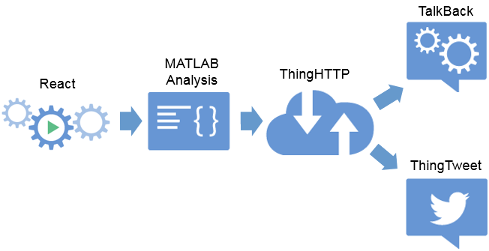
\includegraphics[width=.5\textwidth]{fig8.png}
		\caption{Exemplo de uso do Thingspeak}
		\label{fig:arqthings}
	\end{figure}
	
	
	Para iniciar um prot\'otipo na ferramenta~\cite{KRISHNA2014}, \'e necess\'ario uma das seguintes placas de prototipagem: Arduino(com shield de Ethernet ou Wi-Fi), Particle Core/Photon/Electron, Raspberry PI ou Electric Imp; conectadas \`a Internet e configurados com a biblioteca pr\'opria do Thingspeak que far\'a a comunica\c{c}\~ao com os servidores remotos atrav\'es de opera\c{c}\~oes GET e POST do protocolo HTTP.
	
	Ao configurar dispositivos para conectar ao ThingSpeak, os usu\'arios ter\~ao dispon\'iveis as seguintes funcionalidades para trabalhar:
	\begin{labeling}{Event scheduling}
		\item[Data collection] Criar novos canais para coleta dos dados que ser\~ao analizados.
		\item[Open API] APIs REST dispon\'iveis para gest\~ao e publica\c{c}\~ao remota de feeds, canais e a\c{c}\~oes.
		\item[Alerts] Apps dispon\'iveis para monitorar e notificar ocorr\^encia de eventos.
		\item[Event scheduling] App para controle de acionamento de a\c{c}\~oes com base em regras temporais pr\'e-definidas.
		\item[MATLAB] ()analytics and visualizations) App para an\'alise de dados e elimina\c{c}\~ao de "Outliers" em um canal usando fun\c{c}\~oes do MatLab.
		\item[MQTT] (publish support)APIs MQTT dispon\'iveis para publica\c{c}\~ao de mensagens nos Feeds pelo broker MQTT.
		\item[App integrations] Integrar canais de coleta aos apps de transforma\c{c}\~ao dos dados, acionamento de a\c{c}\~oes e visualiza\c{c}\~ao.
	\end{labeling}
	
	O Thingspeak integrado aos recursos do MatLab se mostra uma ferramenta muito adequada para criar fluxos de notifica\c{c}\~ao e controle automatizado a partir da minera\c{c}\~ao dos dados provenientes de uma rede de sensores conectados \`a Web que exija c\'alculos matem\'aticos no processamento, mantendo um alto rendimento. H\'a ainda a possibilidade de utiliza\c{c}\~ao dos recursos de processamento e a\c{c}\~ao do Thingspeak, para cria\c{c}\~ao de regras de intelig\^encia computacional para uso em projetos voltados \`a Intelig\^encia Ambiental, Intelig\^encia Artificial e SWoT. 

%\subsection{instructables}
%\subsection{code project}
%\subsection{channel9}

\subsection{Pachube/Xively}
	Inicialmente criada com o objetivo de se tornar uma rede social para a Internet das Coisas, dando suporte para comunidades virtuais criarem uma infraestrutura de dados compartilhados, foi adquirida pela empresa LogMeIn em 2011, passando a ser um servi\c{c}o de plataforma para a Internet das Coisas, com objetivo de disponibilizar uma plataforma onde voc\^e pode criar produtos conectados que s\~ao operados (Figura~\ref{fig:arqxively}), controlados e automatizados de forma simples utilizando a internet e viabilizando a identifica\c{c}\~ao de insights dos usu\'arios a partir da an\'alise dos dados.
	
	\begin{figure}[ht]
		\centering
		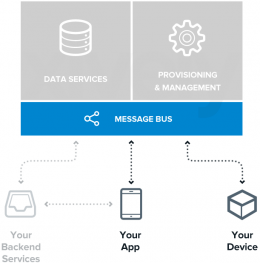
\includegraphics[width=.5\textwidth]{fig7.png}
		\caption{Arquitetura do Xively}
		\label{fig:arqxively}
	\end{figure}
	
	
	Segundo o site da plataforma ~\cite{XIVELY} esses s\~ao os 7 elementos para se criar um produto conectado na Internet das Coisas:
	
	\begin{itemize}
		\item Conceitualizar e definir produto conectado
		\item Fazer prova de conceito com hardware (Seguran\c{c}a)
		\item Desenvolver apps onde usu\'arios podem monitorar seu dispositivo
		\item Habilitar plataforma onde empresa inclui e gerencia seus dispositivos conectados
		\item Integrar dados de dispositivo com ferramenta de relacionamento com clientes 
		\item Preparar ferramenta de an\'alise dos dados para obter insight de usu\'arios
		\item Criar novos canais de engajamento dos usu\'arios ao produto
	\end{itemize}
	
	Alguns exemplos de produtos conectados na plataforma seriam: 
	\begin{labeling}{M\'aquina de lavar}
		\item[M\'aquina de lavar] Identificaria a ocorrencia de algum problema, solicite as pe\c{c}as v\~ao precisar reparo na f\'abrica, chame o t\'ecnico informando a falha identificada e notifique o dono sobre a falha e quanto vai custar o conserto. 
		\item[Carro] Identificaria a hora de uma revis\~ao, verifique a agenda do cliente e cruze com as datas dispon\'iveis na concession\'aria, agendando o melhor hor\'ario, informando a manuten\c{c}\~ao necess\'aria e o custo.
	\end{labeling}

\subsection{IFTTT}
	A concep\c{c}\~ao essencial dessa plataforma \'e automatizar "coisas" utilizando condi\c{c}\~oes(Figura~\ref{fig:ifttt}), assim como o significado de seu acr\^onimo diz: "Se acontecer isso, ent\~ao fa\c{c}a aquilo" (If This, Then That). Ele \'e tanto um website como um app mobile lan\c{c}ado em 2010 com o slogan "Coloque a internet para trabalhar para voc\^e" e com objetivo de automatizar tudo o que for poss\'ivel, desde tarefas nos seus apps e sites favoritos at\'e gadgets e dispositivos inteligentes. A plataforma possui 4 elementos.
	
	\begin{labeling}{Receitas/Applets}
		\item[Gatilhos] "Se" da condi\c{c}\~ao desejada
		\item[A\c{c}\~oes] "Aquilo" da condi\c{c}\~ao desejada
		\item[Receitas/Applets] Condi\c{c}\~oes, ou uni\~ao de um trigger com uma action
		\item[Canais/Servi\c{c}os]  Descri\c{c}\~ao dos dados de um certo servi\c{c}o
	\end{labeling}
	
	Atualmente a plataforma suporta mais de 110 servi\c{c}os ("canais") incluindo apps para dispositivos Android e Apple iOS como Lembretes e Fotos, e tamb\'em sites web como Facebook, Instagram, Flickr, Tumblr, Google Calendar, Google Drive, Feedly, Foursquare, LinkedIn, SoundCloud, WordPress, YouTube, e muitos outros.
	
	\begin{figure}[ht]
		\centering
		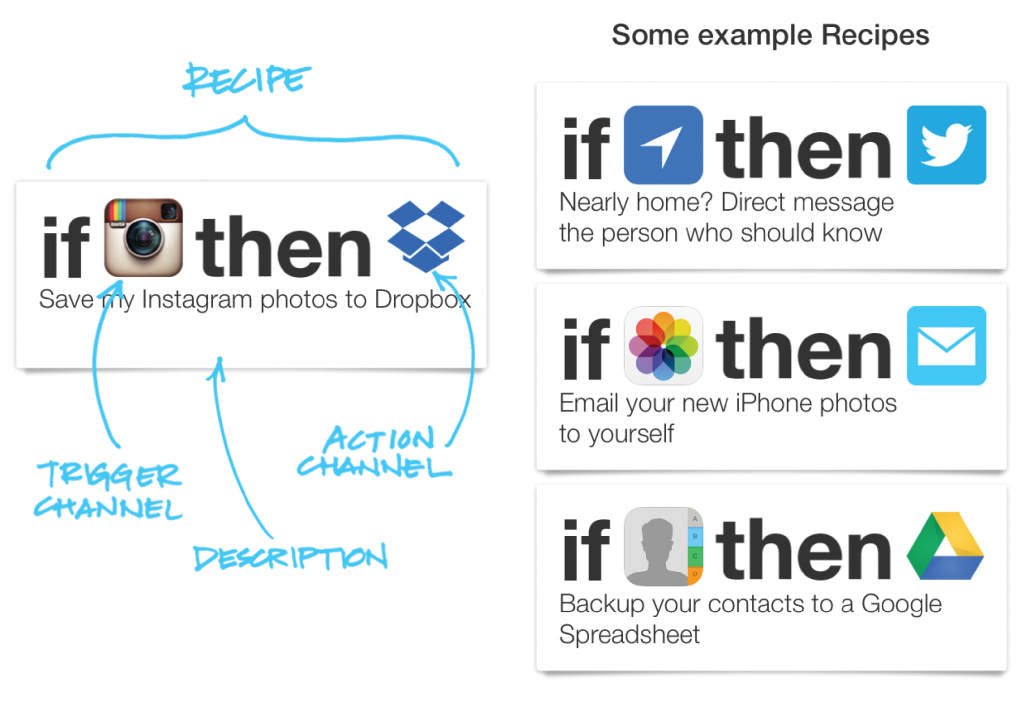
\includegraphics[width=.5\textwidth]{fig5.png}
		\caption{Exemplo de automatiza\c{c}\~ao no IFTTT}
		\label{fig:ifttt}
	\end{figure}
	
	diminuir a sua perda de tempo, automatizandos todas as "coisas" poss\'iveis e criando canais onde voc\^e possa verificar as informa\c{c}\~oes que precisa.  com tantas "coisas" virtuais no mundo querendo tomar a sua aten\c{c}\~ao, porqu\^e n\~ao automatizar tudo o que for poss\'ivel e caso seja realmente necess\'ario a sua aten\c{c}\~ao, voc\^e seja 
	
 %Temas técnicos relacionados ao trabalho

\chapter{Proposta de trabalho que será desenvolvida}
\section{Outros aspectos que impactam a parte principal descrita anteriormente} 5pg
\subsection{sub-item x} %Outros aspectos que impactam a parte principal descrita anteriormente

\chapter{Tecnologias Utilizadas}
\section{Desenvolvimento}
	\subsection{NodeJS}
	\subsection{AngularJS}
	\subsection{Material Design}
	\subsection{Plugins JS}
		\paragraph{Johnny5} 
		\paragraph{Genisys}
		\paragraph{AngularFire}
		\paragraph{AngularMaterial}
	\section{Cloudmqtt}
		\subsection{MQTT}
	\section{Firebase}
		\subsection{Database/ Pub-Sub}
	\section{Prot\'otipos}
		\subsection{Arduino}
		\subsection{NodeMCU}
		\subsection{Firmata firmware}
	\section{Sensors}
	\subsection{sub-item x}
	\section{Processamento dos dados}
		\subsection{Apache Kafka}
		Ferramenta projetada para funcionar como um midleware de mensageria (Figura~\ref{fig:arqkafka}), utilizando o padr\~ao Publish/Subscribe para criar canais ("streams") de mensagens entre v\'arias origens diferentes ("Producers") e os v\'arios destinos inscritos ("Consumers").
		
		\begin{figure}[ht]
			\centering
			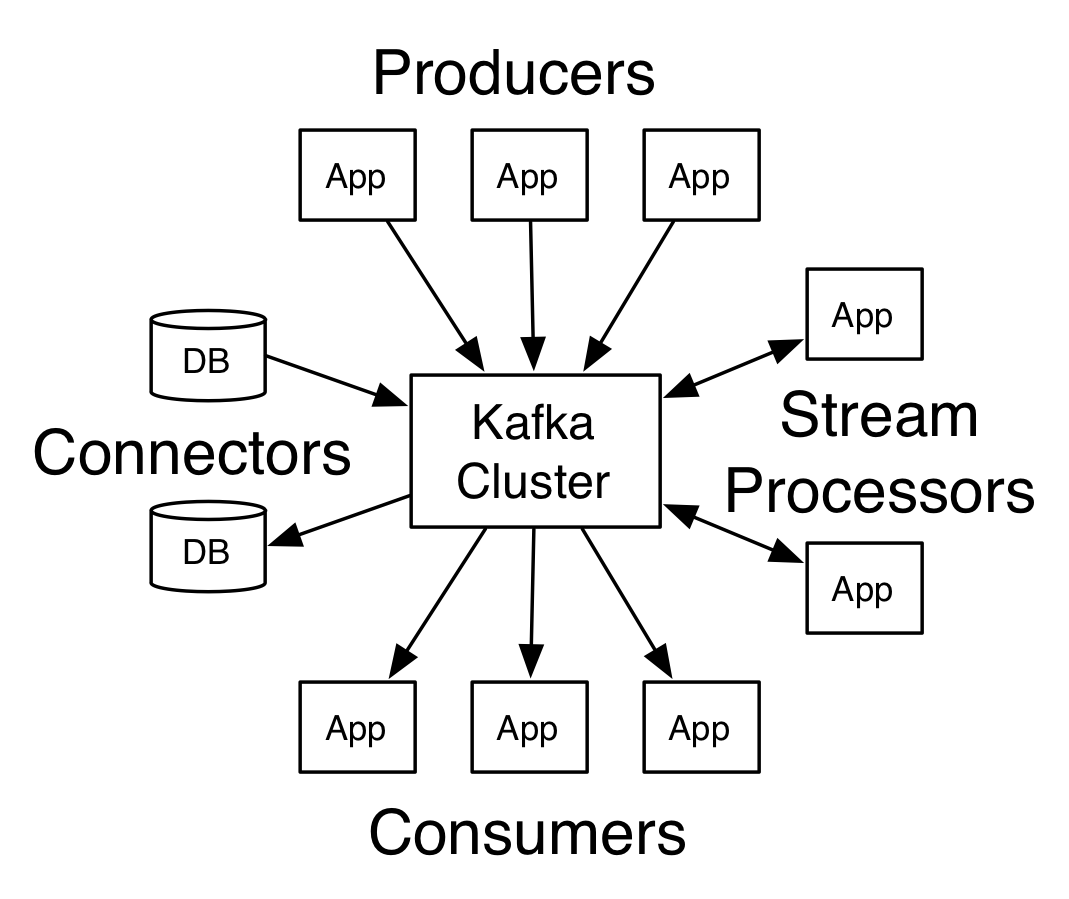
\includegraphics[width=.5\textwidth]{fig0.png}
			\caption{Arquitetura do Kafka}
			\label{fig:arqkafka}
		\end{figure}
		
		Com a utiliza\c{c}\~ao de conectores, bancos de dados podem ser utilizados para persist\^encia de mensagens e ao conect\'a-lo à ferramentas de \'analise e processamento de dados ("Stream Processors"), suas mensagens podem ser transformadas antes de sua publiblica\c{c}\~ao.
		
		Dentre os principais benef\'icios da ferramenta est\~ao: publica\c{c}\~ao em tempo real, funcionamento distribu\'ido em um ou mais servidores, separa\c{c}\~ao dos canais em categorias/t\'opicos, possui recursos de particionamento tolerantes à falhas e garantia na entrega das mensagens com replica\c{c}\~ao de dados. 
		
		\subsection{Apache Storm}
		Essa ferramenta Open Source pode ser utilizada na execu\c{c}\~ao de tarefas em paralelo de forma continua, que \'e o caso de grande parte dos projetos de IoT. Seus Fluxos de trabalhos ou "Topologias", devem ser projetados a partir de grafos ac\'iclicos direcionados (DAG's) que ao entrar em execu\c{c}\~ao, realizam suas tarefas indefinidamente processando os dados gerados pelos dispositivos ub\'iquos de forma cont\'inua. Suas topologias s\'o param de rodar em 2 casos, a partir da interven\c{c}\~ao do usu\'ario matando seu processo ou na ocorr\^encia de uma falha irrecuper\'avel. 
		
		Sua topologia \'e formada por "spouts" ou "bolts" como seus v\'ertices, enquanto que suas arestas representam fluxos de dados trafegados entre os n\'os do grafo. Em conjunto, v\'ertices e arestas da topologia agem como um pipeline de transforma\c{c}\~ao dos dados em tempo real(Figura~\ref{fig:arqstorm}).
		
		\begin{figure}[ht]
			\centering
			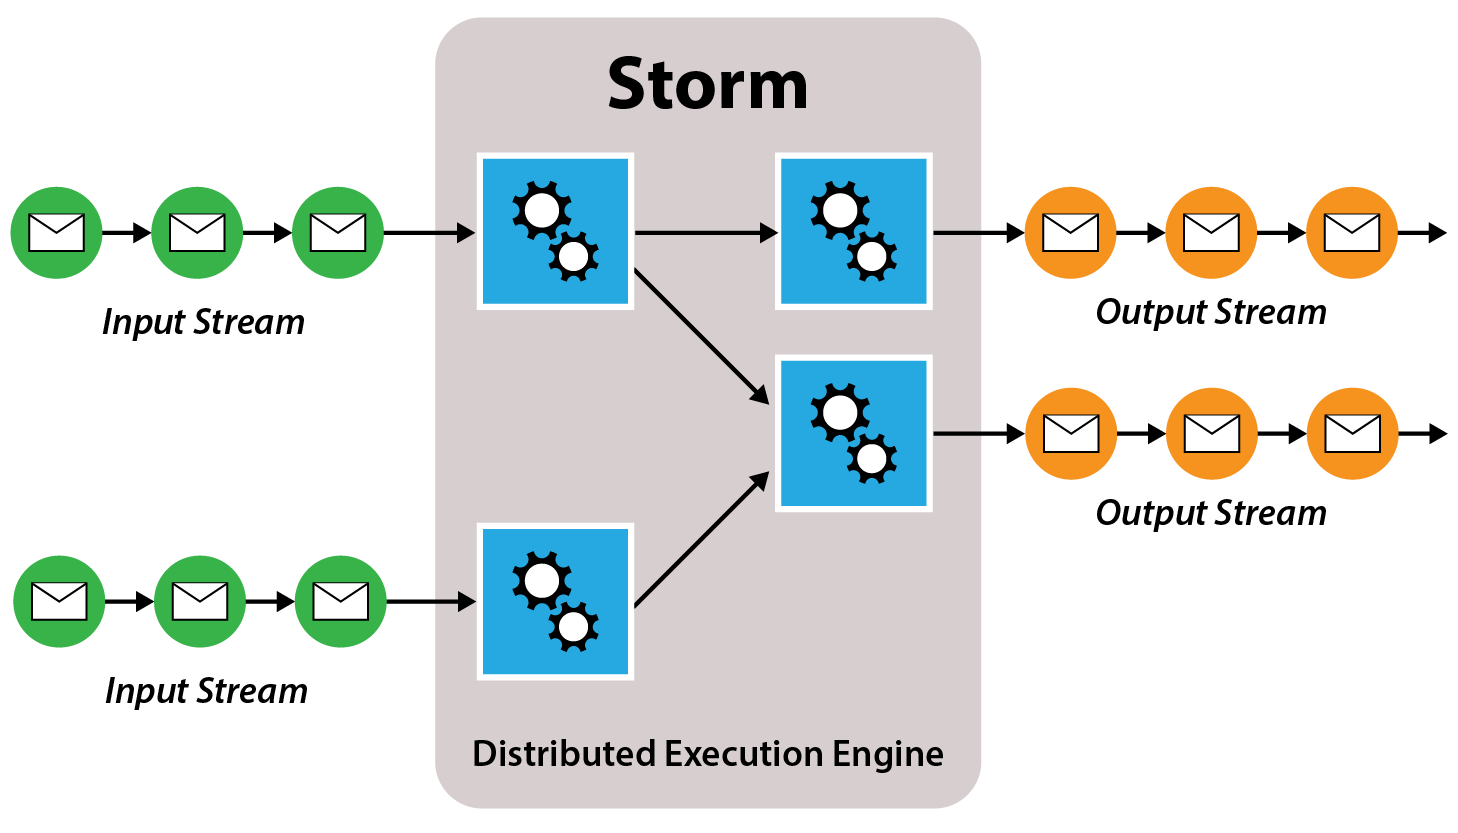
\includegraphics[width=.5\textwidth]{fig4.png}
			\caption{Exemplo de topologia no Storm}
			\label{fig:arqstorm}
		\end{figure}
		
		O Storm n\~ao possui suporte nativo aos clusters do Hadoop/YARN (Ainda em desenvolvimento), ao inv\'es disso ele usa a estrutura da ferramenta Zookeeper e seus pr\'oprios processos de trabalho (master/minion) para coordena\c{c}\~ao de suas topologias, estados e mensagens sem\^anticas de garantia. Al\'em disso, ele pode consumir e escrever arquivos no HDFS e tamb\'em rodar nativamente sobre o gerenciador de cluster Apache Mesos ou com o suporte da plataforma de orequestra\c{c}\~ao de containers Marathon. %Proposta de trabalho que será desenvolvida

\chapter{Conclus�o}\label{cap:conclusao}
Concluindo, podemos ver que todas os paradigmas analisados possuem grande sinergia, por�m analisando mais atentamente, vemos que na verdade a grande semelhan�a entre elas tem como origem o fato de serem ramifica��es da Computa��o Ub�qua. Podemos resumir a  diferan�a entre os paradigmas por suas principais propostas, da seguinte forma: 

\begin{labeling}{Disappearing Computing}
	\item[Computa��o Ub�qua] Aprimorar dispositivos ao ponto que sua utiliza��o se tornar� impercept�vel.
	\item[Disappearing Computing] Definir tecnologias respons�veis pela transforma��o de computadores em objetos impercept�veis no ambiente.
	\item[Internet das Coisas] Unir dispositivos e sensores criando uma rede de dispositivos ub�quos.
	\item[Web das Coisas] Garantir que dispositivos ub�quos heterog�neos possam se localizar e interagir na internet de forma transparente.
	\item[Web Social das Coisas] Explorar redes sociais incluindo dispositivos ub�quos que consigam interpretar e serem interpretados corretamente entre si e com as pessoas.
\end{labeling}

Por fim, novos projetos, eventos, apresenta��es e not�cias sobre esses paradigmas s�o inclu�dos di�riamente na internet por pesquisadores e entusiastas no assunto. Ao avaliar seus pr�ximos passos, busque distinguir paradigmas e tecnologias que sendo pesquisadas no momento, identificando assim o caminho prov�vel para as novas oportunidades e desafios.

\bibliography{referencias} % bibname=nome do seu arquivo BibTeX

%% DICA: voce pode ir definindo os acronimos ao longo do texto.
%% Por exemplo, no capitulo 1, vc ta escrevendo:
%% Segundo Fulano, Model-Driven Development (MDD)\acronym{MDD}{Model-Driven Development} ? uma t?cnica bla bla bla...
%\acronym{MDD}{Model-Driven Development}
\listofacronyms

\apendice

\anexo
	
\end{document}